\documentclass{article}

%% Created with wxMaxima 12.01.0

\setlength{\parskip}{\medskipamount}
\setlength{\parindent}{0pt}
\usepackage[utf8]{inputenc}
\usepackage{graphicx}
\usepackage{color}
\usepackage{amsmath}

\definecolor{labelcolor}{RGB}{100,0,0}

\begin{document}

\noindent
%%%%%%%%%%%%%%%
%%% INPUT:
\begin{minipage}[t]{8ex}{\color{red}\bf
\begin{verbatim}
(%i1) 
\end{verbatim}}
\end{minipage}
\begin{minipage}[t]{\textwidth}{\color{blue}
\begin{verbatim}
w:2*%pi*50;
R:12;
L:22*10^-3;
z:sqrt(R^2+(w*L)^2),numer;
b:atan(L*w/R);
Vm:230*sqrt(2);
E:180;
a:30*(%pi/180);
V(t):=Vm*sin(w*t+a);
C1:((Vm/L*1/((R/L)^2+w^2))*(w*cos(a)-(R/L)*sin(a))+E/R),numer;
C2:(Vm/L*1/((R/L)^2+w^2)*((R/L)*sin(a)-w*cos(a))),numer;
C3:(Vm/L*1/((R/L)^2+w^2)*((R/L)*cos(a)+w*sin(a))),numer;
C4:(E/R)-Vm/z*sin(a-b),numer;
\end{verbatim}}
\end{minipage}
%%% OUTPUT:
\begin{math}\displaystyle
\parbox{8ex}{\color{labelcolor}(\%o1) }
100\,\pi 
\end{math}

\begin{math}\displaystyle
\parbox{8ex}{\color{labelcolor}(\%o2) }
12
\end{math}

\begin{math}\displaystyle
\parbox{8ex}{\color{labelcolor}(\%o3) }
\frac{11}{500}
\end{math}

\begin{math}\displaystyle
\parbox{8ex}{\color{labelcolor}(\%o4) }
13.84806431604333
\end{math}

\begin{math}\displaystyle
\parbox{8ex}{\color{labelcolor}(\%o5) }
\mathrm{atan}\left( \frac{11\,\pi }{60}\right) 
\end{math}

\begin{math}\displaystyle
\parbox{8ex}{\color{labelcolor}(\%o6) }
115\,{2}^{\frac{3}{2}}
\end{math}

\begin{math}\displaystyle
\parbox{8ex}{\color{labelcolor}(\%o7) }
180
\end{math}

\begin{math}\displaystyle
\parbox{8ex}{\color{labelcolor}(\%o8) }
\frac{\pi }{6}
\end{math}

\begin{math}\displaystyle
\parbox{8ex}{\color{labelcolor}(\%o9) }
\mathrm{V}\left( t\right) :=Vm\,\mathrm{sin}\left( w\,t+a\right) 
\end{math}

\begin{math}\displaystyle
\parbox{8ex}{\color{labelcolor}(\%o10) }
14.97547008795629
\end{math}

\begin{math}\displaystyle
\parbox{8ex}{\color{labelcolor}(\%o11) }
0.024529912043714
\end{math}

\begin{math}\displaystyle
\parbox{8ex}{\color{labelcolor}(\%o12) }
23.48840491677491
\end{math}

\begin{math}\displaystyle
\parbox{8ex}{\color{labelcolor}(\%o13) }
14.97547008795629
\end{math}
%%%%%%%%%%%%%%%


\noindent
%%%%%%%%%%%%%%%
%%% INPUT:
\begin{minipage}[t]{8ex}{\color{red}\bf
\begin{verbatim}
(%i14) 
\end{verbatim}}
\end{minipage}
\begin{minipage}[t]{\textwidth}{\color{blue}
\begin{verbatim}
i1(t):=C1*%e^(-R/L*t)+C2*cos(w*t)+C3*sin(w*t)-(E/R);
i2(t):=C4*%e^(-R/L*t)+Vm/z*sin(w*t+a-b)-(E/R);
wxplot2d([i1(t),i2(t)],[t,-0.001,0.04],[y,-40,10],[gnuplot_preamble, "set grid"]);
\end{verbatim}}
\end{minipage}
%%% OUTPUT:
\begin{math}\displaystyle
\parbox{8ex}{\color{labelcolor}(\%o14) }
\mathrm{i1}\left( t\right) :=C1\,{e}^{\frac{-R}{L}\,t}+C2\,\mathrm{cos}\left( w\,t\right) +C3\,\mathrm{sin}\left( w\,t\right) -\frac{E}{R}
\end{math}

\begin{math}\displaystyle
\parbox{8ex}{\color{labelcolor}(\%o15) }
\mathrm{i2}\left( t\right) :=C4\,{e}^{\frac{-R}{L}\,t}+\frac{Vm}{z}\,\mathrm{sin}\left( w\,t+a-b\right) -\frac{E}{R}
\end{math}

\begin{math}\displaystyle
\parbox{8ex}{\color{labelcolor}(\%t16) }
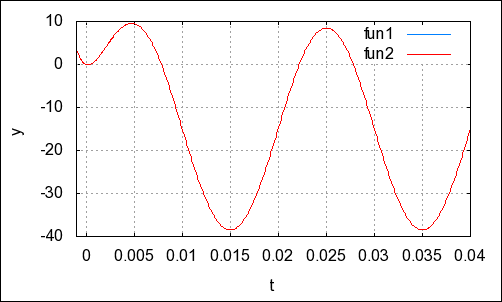
\includegraphics[width=9cm]{proof_2_img/proof_2_1.png}
\end{math}

\begin{math}\displaystyle
\parbox{8ex}{\color{labelcolor}(\%o16) }
$ $
\end{math}
%%%%%%%%%%%%%%%


\noindent
%%%%%%%%%%%%%%%
%%% INPUT:
\begin{minipage}[t]{8ex}{\color{red}\bf
\begin{verbatim}
(%i17) 
\end{verbatim}}
\end{minipage}
\begin{minipage}[t]{\textwidth}{\color{blue}
\begin{verbatim}
i1(t):=C1*%e^(-R/L*t);
i2(t):=C4*%e^(-R/L*t);
wxplot2d([i1(t),i2(t)],[t,-0.001,0.04],[y,-1,18],[gnuplot_preamble, "set grid"]);
\end{verbatim}}
\end{minipage}
%%% OUTPUT:
\begin{math}\displaystyle
\parbox{8ex}{\color{labelcolor}(\%o17) }
\mathrm{i1}\left( t\right) :=C1\,{e}^{\frac{-R}{L}\,t}
\end{math}

\begin{math}\displaystyle
\parbox{8ex}{\color{labelcolor}(\%o18) }
\mathrm{i2}\left( t\right) :=C4\,{e}^{\frac{-R}{L}\,t}plot2d: some values were clipped.plot2d: some values were clipped.
\end{math}

\begin{math}\displaystyle
\parbox{8ex}{\color{labelcolor}(\%t19) }
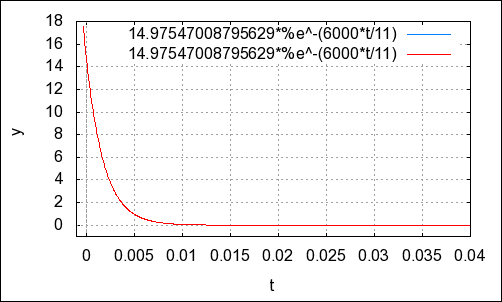
\includegraphics[width=9cm]{proof_2_img/proof_2_2.png}
\end{math}

\begin{math}\displaystyle
\parbox{8ex}{\color{labelcolor}(\%o19) }
$ $
\end{math}
%%%%%%%%%%%%%%%


\noindent
%%%%%%%%%%%%%%%
%%% INPUT:
\begin{minipage}[t]{8ex}{\color{red}\bf
\begin{verbatim}
(%i20) 
\end{verbatim}}
\end{minipage}
\begin{minipage}[t]{\textwidth}{\color{blue}
\begin{verbatim}
i1(t):=C2*cos(w*t)+C3*sin(w*t)-(E/R);
i2(t):=Vm/z*sin(w*t+a-b)-(E/R);
wxplot2d([i1(t),i2(t)],[t,-0.001,0.04],[y,-40,10],[gnuplot_preamble, "set grid"]);
\end{verbatim}}
\end{minipage}
%%% OUTPUT:
\begin{math}\displaystyle
\parbox{8ex}{\color{labelcolor}(\%o20) }
\mathrm{i1}\left( t\right) :=C2\,\mathrm{cos}\left( w\,t\right) +C3\,\mathrm{sin}\left( w\,t\right) -\frac{E}{R}
\end{math}

\begin{math}\displaystyle
\parbox{8ex}{\color{labelcolor}(\%o21) }
\mathrm{i2}\left( t\right) :=\frac{Vm}{z}\,\mathrm{sin}\left( w\,t+a-b\right) -\frac{E}{R}
\end{math}

\begin{math}\displaystyle
\parbox{8ex}{\color{labelcolor}(\%t22) }
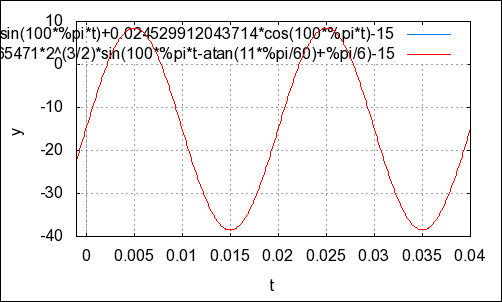
\includegraphics[width=9cm]{proof_2_img/proof_2_3.png}
\end{math}

\begin{math}\displaystyle
\parbox{8ex}{\color{labelcolor}(\%o22) }
$ $
\end{math}
%%%%%%%%%%%%%%%

\end{document}
